% ===== RUBRIC OF TEACHER'S JOB ASPECTS =====

% A single rubric criterion
\newcommand{\rubriccriterion}[4]{
\stepcounter{rubricquestion}
\section*{\therubricquestion: #1}

\smallskip
\note{Neznalý:} #2

\note{Začátečník:} #3

\note{Guru:} #4

\medskip
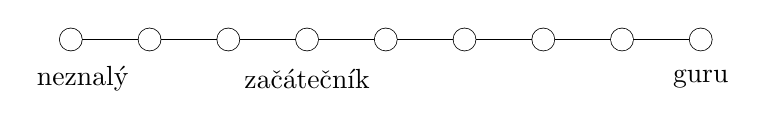
\begin{tikzpicture}
\draw (0,0) -- (8,0);
\foreach \i in {0,1,...,8} % numbers on line
{
\fill[black] (\i,0) circle (1.5 mm);
\fill[white] (\i,0) circle (1.4 mm);
}
\node at (0.15, -0.5) {neznalý};
\node at (3, -0.5)    {začátečník};
\node at (8, -0.5)    {guru};
\end{tikzpicture}
}

\restoregeometry
\chapter*{Učitelská rubrika}
\label{rubric}

Následující strany prezentují rubriku činností učitele. Běžně si učitelé-začátečníci (a někdy ani učitelé-veteráni) neuvědomují všechny úrovně a dimenze učitelského umění. To se často stává proto, že se s tím nikdy nesetkali u ostatních. Je možné, že po pár měsících či letech učení přijde moment, kdy si uvědomíte, že máte mnohem větší prostor pro zlepšování, než jste si prvně mysleli\punct{.}\footnote{Více informací najdete například v knize \emph{How Learning Works: Seven Research-Based Principles for Smart Teaching}.}

\section*{Co je to rubrika?}

Rubrika je nástroj pro \emph{self-assessment} (uvědomění a popsání svých vlastních znalostí a dovedností). Pomáhá zřetelně si uvědomit a pojmenovat, jaké části daný koncept má (např.\ umět programovat znamená být schopen navrhnout algoritmus, efektivně pracovat s~pamětí, znát syntaxi, \dots). Zároveň umožňuje vyhodnotit vlastní úroveň v jednotlivých částech (např.\ navrhnout algoritmus umím dobře, zapsat to kódem mám trochu problém a práci s pamětí neoptimalizuji vůbec).

\section*{Jak učitelskou rubriku používat?}

Na začátku semestru si rubriku vyplň (označ, kde na dané škále jsou podle tebe tvoje schopnosti). Vyber si 1--3 oblasti, na které se chceš zaměřit v tomto semestru. Chceš-li být hodně důsledný(á), můžeš vymyslet i konkrétní kroky, které uděláš, a indikátory svého postupu. Na konci semestru si můžeš rubriku vyplnit znovu a vyhodnotit, v čem jsi se posunul(a).

Rubriku můžeš čist i jako manifest -- popisy kategorie \enquote{guru} vystihují naši představu o tom, co zvládají skvělí učitelé a k čemu bychom rádi vedli začínající učitele.

\newcounter{rubricquestion}

\newpage
\rubriccriterion{Cíle hodiny, vědomá pozornost}
{Ve výuce nemám jasně stanovené cíle. Když učím, nevnímám, co se děje a kam směřujeme. Často se cítím ztracen(a).}
{Někdy se mi daří uvědomovat si, jaký mám cíl, co právě dělám a jaký to bude mít efekt. Většinou ale nemám při výuce vědomou pozornost.}
{Během výuky jsem si téměř vždy vědom(a) toho, jaký cíl sleduji, co se se mnou i se skupinou děje, co dělám a jaký to bude mít efekt. Vím, jak jsme se dostali tam, kde právě jsme.}

\rule{\textwidth}{0.4pt}
\rubriccriterion{Interakce se skupinou, kladení otázek skupině}
{Se skupinou neinteraguji. Neptám se, protože bych asi nedostal(a) odpověď. Nevím, jak studenty zapojit.}
{Vím, že lze interagovat se skupinou a znám nástroje (chápu, jak by to šlo). Nedokážu je ale dobře používat. Někdy  se skupiny ptám, ale nedostávám odpověď.}
{Se skupinou často a efektivně interaguji. Ptám se způsobem, který studenty aktivizuje a zapojuje. Situace, kdy nedostávám od skupiny odpověď dokážu obratně řešit (např.\ přeformulováním otázky).}

\newpage
\rubriccriterion{Strukturování výuky}
{O strukturování výuky vůbec nepřemýšlím.}
{Chápu smysl přehledného strukturování své hodiny a snažím se o to. Často se ale zamotám, ztratím nit, nebo řeším více věcí naráz a studenti se pak ztrácí nebo odpojují.}
{Moje hodiny mají jasnou strukturu. Studenti ví, co se právě děje, co bude následovat a chápou návaznosti. Mezi jednotlivými bloky vědomě dělám zřetelné přechody.}

\rule{\textwidth}{0.4pt}
\rubriccriterion{Vlastní pocity a spokojenost s výukou}
{Jsem nespokojen(a) se svými hodinami anebo své pocity a vlasní spokojenost s výukou nijak nereflektuji. Netěším se do výuky.}
{Ve výuce si často moc nevěřím. Někdy mi vyjdou části hodiny, ale často se cítím napjatě nebo mám strach, že něco pokazím.}
{Ve výuce se cítím uvolněně a sebevědomě. Baví mě to a mám svůj styl.}

\newpage
\rubriccriterion{Formativní zpětná vazba}
{O dávání osobní zpětné vazby studentům nijak nepřemýšlím.}
{Snažím se studentům zpětnou vazbu dávat, aby mohli růst. Myslím si však, že jí není dost, nebo to nedělám efektivně. Studenti mou zpětnou vazbu někdy nevnímají jako podporu a projev respektu.}
{Se studenty ve výuce interaguji tak, že dostávají průběžně formativní zpětnou vazbu. Chápou tedy, co jim jde, kde dělají chyby a jak se mohou zlepšovat. Zároveň cítí, že je respektuji a zpětné vazby se nebojí.}

\rule{\textwidth}{0.4pt}
\rubriccriterion{Jasné zadávání pokynů a úloh}
{O tom, jak zadávat pokyny nebo úlohy, nijak zvlášť nepřemýšlím.}
{Stává se mi, že zadám pokyn nebo úlohu a studenti neví, co dělat, jak začít nebo k čemu mají dojít (co má být výsledkem).}
{Když zadávám pokyn nebo úlohu, studenti mají jasno v~tom, co dělat, jak začít nebo k čemu mají dojít.}

\newpage
\rubriccriterion{Variabilita a inovace ve výuce}
{Učím tak, jak mi řekli nebo kopíruji výuku, kterou jsem zažil(a). Nepřemýšlím o~jiných variantách.}
{Jsem si vědom(a) toho, že existuje mnoho typů aktivit, které lze při výuce použít. Neznám jich ale dostatek, nedokážu je efektivně zadávat, nebo nemám jasno v tom, proč je používat.}
{Znám mnoho různých aktivit a svou výuku skládám tak, aby byla dostatečně pestrá. Vybrané aktivity efektivně procvičují to, co mám záměr procvičovat. Zároveň studenty efektivně zapojují a zvyšují jejich motivaci se učit.}

\rule{\textwidth}{0.4pt}
\rubriccriterion{Širší kontext mé výuky}
{O širším kontextu výuky a mého kurzu nepřemýšlím.}
{Je pro mě těžké jasně pojmenovat znalosti a dovednosti, které u~studentů rozvíjím. Nevím, v jakém kontextu je studenti využijí. Nevidím propojení s dalšími kurzy.}
{Mám jasnou představu o tom, k čemu studenty vedu (jaké dovednosti rozvíjím, jaké znalosti chci předat). Vím, proč tyto dovednosti rozvíjím a v jakém kontextu je studenti v budoucnu použijí. Vidím širší kontext.}
\vspace*{-1em}

\newpage
\rubriccriterion{Jasné vysvětlování}
{Svoje způsoby vysvětlování nijak nereflektuji.}
{Když vysvětluji, běžně se mi stává, že si nejsem jistý, zda vysvětluji dobře a zda to studentům pomáhá při pochopení.}
{Když vysvětluji teorii, demonstruji řešení a efektivně opravuji chyby. Dokážu se dobře vžít do toho, jak to vidí student. Moje vysvělování efektivně pomáhá studentům pochopit problém. Nestává se mi, že bych vysvětloval(a) něco, na co se neptali.}

\rule{\textwidth}{0.4pt}
\rubriccriterion{Nastavení prostředí, systémy ve výuce}
{O atmosféře ve výuce nepřemýšlím. Systémy ve své výuce nevnímám.}
{Přemýšlím o nastavení pravidel i atmosféry. Systémy ve výuce (např.\ bodování) přebírám od ostatních. Nemám ale jasno v jejich efektech, nebo neznám způsoby, jak je lze upravit.}
{Umím ve výuce vytvořit prostředí, které podporuje efektivní učení. U systémů, které používám (např.\ bodování, bonbóny, zahajovací rituály) chápu efekt. Systémy nepřebírám slepě, chápu jejich účel a uzpůsobuji podle svých potřeb.}

\newpage
\rubriccriterion{Flexibilita, přizpůsobování výuky na místě}
{Na situace vzniklé v průběhu výuky nijak vědomě nereaguji.}
{Uvědomuji si chvíle, kdy by mohlo být zajímavé nebo užitečné dělat něco jiného, než jsem měl(a) v plánu. Většinou ale nedokážu v daný moment vhodně zareagovat.}
{Dokážu svoji výuku průběžně přizpůsobovat tomu, co se právě děje ve skupině a co studenti potřebují. Mám k tomu dostatek nástrojů a dokážu je efektivně použít.}

\rule{\textwidth}{0.4pt}
\rubriccriterion{Individuální interakce se studenty}
{O konzultacích nebo jiných indidivuálních interakcích nijak vědomě nepřemýšlím.}
{Stává se mi, že si často nevím rady při individuální interakci se studentem (např.\ zkoušení u~tabule, konzultace). Interakce neprobíhá efektivně nebo se student cítí zastrašen.}
{Při interakcích s jednotlivci (např.\ zkoušení, konzultace) efektivně využívám čas. Studenti se mnou konzultují rádi a je to pro ně užitečné. Cítí ze mě respekt a podporu.}

\newpage
\rubriccriterion{Skupinová práce, management skupiny}
{Přijde mi, že dělit skupinu je zbytečnost. O~práci v~menších skupinkách nepřemýšlím.}
{Uvědomuji si možnosti práce ve dvojicích či menších skupinách. Tuším, že bych toho mohl(a) lépe využívat, hledám jak.}
{Mám jasno v tom, kdy chci pracovat s celou skupinou, kdy s jednotlivci a kdy se skupinkami. Rozdělení do menších skupin efektivně používám, když je to potřeba. Ve vhodných případech zadávám interakce mezi skupinami.}

\rule{\textwidth}{0.4pt}
\rubriccriterion{Čtení atmosféry ve skupině}
{Skupinu ve své výuce nesleduji, pozornost věnuji pouze obsahu.}
{Uvědomuji si, že mi skupina vysílá signály a že by bylo dobré jim rozumět a využít je pro efektivní vedení výuky. Ve výuce to ale dokážu jen výjimečně.}
{Dokážu dobře odhadnout naladění skupiny. Mám jasno v tom, co se ve skupině studentů děje (např. únava, nadšení, obava).}
